\subsection{A sharper whole-space square and all six intermediate phases}
\label{sec:atomic-square-12}

The later full-space verification improves the electronic complement itself,
rather than enlarging a finite angular cutoff. Put $e=U/|U|$ and $A=g|U|$
when $U\ne0$. The bounded proof field
\begin{equation}
 F(x)=\frac{A}{4\tau}\{2(e\cdot n)n-e\}
\label{eq:point-proof-field-12}
\end{equation}
has $|F|^2=A^2/(16\tau^2)$ and
$\operatorname{div}F=(A/\tau)(e\cdot n)/r$. Its flux through a shrinking
sphere tends to zero. For a smooth compactly supported test function,
integration by parts gives
\begin{equation}
 \langle\psi,h_A\psi\rangle
 =\tau\|\nabla\psi+F\psi\|^2
       -\frac{A^2}{16\tau}\|\psi\|^2.
\end{equation}
The Coulomb form bound and density extend this identity to the full $H^1$
form domain. The $A=0$ case is the free kinetic form. Summing before
restricting to the antisymmetric space proves
\begin{equation}
 h_A\ge-\frac{A^2}{16\tau},\qquad e_n\ge-\frac n{16}.
\label{eq:point-sixteenth-12}
\end{equation}
No equality state or optimality of the constant is inferred. This is the
factor-four improvement over the earlier $-n/4$ comparison, with every
radial and angular direction still present.\samref{REF12_ATOMS}

The companion 72-function logarithmic-cusp trial retains its complete
physical overlap matrix. Its corrected one-electron Ritz value and
six-electron Slater trace are, respectively,
\begin{align*}
 -0.04735264960221189793807378413284,\\
 -0.16329578569671925116100439108172.
\end{align*}
Tiny overlaps are retained before normalization. For phase guarantees it
is enough to use the following conservative positive rational strengths
$a_n$, meaning an electronic upper $e_n\le-a_n$:
\begin{equation}
\begin{split}
(a_1,a_2,a_3)={}&(2367/50000,9469/100000,5767/50000),\\
(a_4,a_5,a_6)={}&(13599/100000,3741/25000,16329/100000).
\end{split}
\end{equation}
Writing $\chi=g^2/\tau$, each carbon-343 intermediate phase now has the
nonempty sufficient interval
\begin{equation}
 \frac{35}{24a_n}<\chi<\frac{1968}{17n},\qquad n=1,\ldots,6.
\label{eq:343-all-six-12}
\end{equation}
Indeed $a_n\chi>35/24$ forces entry past the first nuclear transition,
while $(n/16)\chi<123/17$ keeps the exact electronic coefficient below
the second. Thus all six formerly unresolved intermediate guarantees
close. The verified roster now has 50 phase/inventory guarantees,
44 populated point-source binding accounts and ten exact empty controls.
For example the six-electron carbon-444 point-source interval becomes
approximately $[23.514,54]$, replacing the earlier $[23.364,216]$.
These are point-source accounts; the interacting finite-core comparison
below has a different Hamiltonian and reference.

\subsection{The finite-core Pauli split and complete carbon minima}
\label{sec:finite-core-12}

For $d_c(r)=\max(r,r_c)$, multiply
\eqref{eq:point-proof-field-12} by
\begin{equation}
 h(r)=\begin{cases}4r/(5r_c),&r\le r_c,\\
                 1-r_c^4/(5r^4),&r\ge r_c.
       \end{cases}
\end{equation}
The profile and its derivative match, its divergence is the original
regularized directional potential, and $0\le h\le1$. Neither an origin
delta nor an interface term is introduced. Put $C=g_cZ$ and
$A=g_p\sqrt q$. Split the same kinetic form into fractions $\theta$ and
$1-\theta$. Complete Coulomb spin-state occupation bounds the scalar part
by $-C^2w_n/(4\theta\tau)$; the directional square bounds the other part
by $-nA^2/[16(1-\theta)\tau]$. Optimizing $0<\theta<1$ gives
\begin{equation}
 E_{e,n}(q)\ge-\frac{[C\sqrt{w_n}+(A/2)\sqrt n]^2}{4\tau}.
\label{eq:core-split-12}
\end{equation}
Endpoint limits cover $C=0$ or $A=0$. The positive original pair form is
discarded only for this lower comparison; the variational upper retains
all direct and exchange entries. Take the maximum of
\eqref{eq:core-split-12}, the preceding scalar comparison and
$-n(C+A)/r_c$ before either complete nuclear minimum. In particular this
does not require $C\ge A$.

In the weak-polarization panel $\tau=r_c=g_c=v_c=1$,
$g_p=v_p=1/10$, complete minimization over the retained $q/I$ roster gives
the current neutral carbon binding uppers in
Table~\ref{tab:carbon-upgrade-12}. The previous fully occupied witnesses
still provide the binding lower endpoints. The new numbers improve the
complement lower, hence the upper on binding; they are not new measured
binding energies.\samref{REF12_ATOMS}

\begin{table}[htbp]\centering\small
\caption{Successive weak-polarization binding uppers, in source units.
The final column uses every original nuclear receiver class.}
\begin{tabular}{lrr}\toprule
Source & Earlier upper & Complete new upper\\\midrule
Carbon 333&32.67&30.9533766184074\\
Carbon 343&34.68&32.3311688245431\\
Carbon 444&38.88&35.1767532368147\\\bottomrule
\end{tabular}\label{tab:carbon-upgrade-12}
\end{table}

For carbon 444 the intrinsic inequality
$I(q)-282\ge(144-q)/3$ locks the minimizing class at $q=144$.
Its final binding upper is exactly
\begin{equation}
 \frac{1377}{50}+\frac{27\sqrt2}{5}=35.1767532368147\ldots.
\end{equation}
The complete replay corrected two earlier rounded energy displays and
the cusp Gram normalization. The rational phase guarantees survive these
corrections. The constant-lapse extension also held, while its former
blanket comparison with the original geometric Pauli bound required a
correction. The exact geometric occupation in Chapter~XV supplies the
appropriate new comparison.

\begin{figure}[htbp]\centering
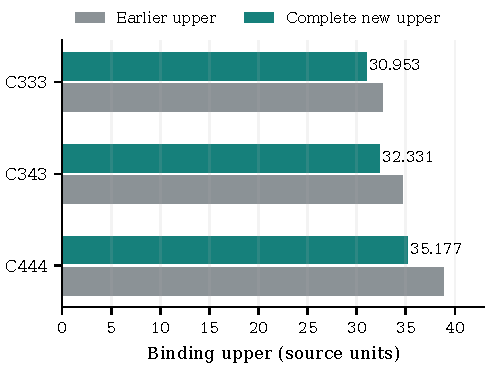
\includegraphics[width=\columnwidth]{refinement_20261112/figures/atomic_bounds.pdf}
\caption{Improvement of the complete weak-polarization carbon binding
uppers. The point-source factor-four bound and the finite-core nuclear
minimization are separate comparisons; this figure shows only the latter.
Data: H003004, complete finite-core replay.}
\label{fig:atomic-bounds-12}
\end{figure}
